\section{统计量的分布}

\subsection{统计量的定义}
样本是进行统计推断的依据,在应用时,往往不是直接使用样本本身,而是针对不同的问题构造样本的适当函数,利用给这些样本的函数进行统计推断,这种样本的函数,就称为统计量。

\begin{BoxDefinition}[统计量]
    设$X_1,X_2,\cdots,X_n$是来自总体$X$的一个样本,而
    \begin{eqnarray}
        g(X_1,X_2,\cdots,X_n)
    \end{eqnarray}
    是$X_1,X_2,\cdots,X_n$的函数,则称$g(X_1,X_2,\cdots,X_n)$是一\uwave{统计量}(Statistic)。
\end{BoxDefinition}

需要指出的是,\empx{统计量本身也是一个随机变量}。因为$X_1,X_2,\cdots,X_n$都是随机变量,而统计量$g(X_1,X_2,\cdots,X_n)$作为随机变量的函数自然也是随机变量。在\xref{sec:两个随机变量的函数的分布}中我们看到,仅仅是两个随机变量的函数的分布就已经非常复杂了,统计量是$n$个随机变量构成的函数,因此可以预期的是,\empx{统计量的分布会非常复杂}。在本小节,我们会首先引入几个重要的统计量。

\begin{BoxDefinition}[样本均值]
    定义\uwave{样本均值}为
    \begin{Equation}
        \xbar{X}=\frac{1}{n}\Sum[k=1][n]X_k
    \end{Equation}
\end{BoxDefinition}

\begin{BoxDefinition}[样本方差]
    定义\uwave{样本方差}为
    \begin{Equation}
        S^2=\frac{1}{n-1}\Sum[k=1][n](X_k-\xbar{X})^2
    \end{Equation}
    定义\uwave{样本标准差}为
    \begin{Equation}
        S=\sqrt{S^2}
    \end{Equation}
\end{BoxDefinition}

这里需要说明的是,或许我们会认为,样本均值$\xbar{X}$和样本方差$S^2$在形式上,看起来与离散型随机变量的均值$E(X)$和方差$D(X)$很相似,但应注意$S^2$前是$1/(n-1)$而非$1/n$!这是有意为之的,因为后面我们会看到,只有这样,样本方差$S^2$才能作为方差$D(X)$的无偏估计。\goodbreak

这里有一个更便捷的样本方差计算公式
\begin{BoxFormula}[样本方差]
    样本方差可用以下公式计算
    \begin{Equation}
        S^2=\frac{1}{n-1}\qty[\Sum[k=1][n](X_k^2)-n\xbar{X}^2]
    \end{Equation}
\end{BoxFormula}
\begin{Proof}
    根据\fancyref{def:样本方差}
    \begin{Equation}&[1]
        S^2=\frac{1}{n-1}\qty[\Sum[k=1][n](X_k-\xbar{X})^2]
    \end{Equation}
    展开平方
    \begin{Equation}&[2]
        S^2=\frac{1}{n-1}\qty[\Sum[k=1][n]X_k^2-2X_k\xbar{X}+\xbar{X}^2]
    \end{Equation}
    而考虑到$\xbar{X}$是常数
    \begin{Equation}&[3]
        S^2=\frac{1}{n-1}\Sum[k=1][n]X_k^2-\frac{2\xbar{X}}{n-1}\Sum[k=1][n]X_k+\frac{n\xbar{X}^2}{n-1}
    \end{Equation}
    根据\fancyref{def:样本均值}
    \begin{Equation}
        S^2=\frac{1}{n-1}\Sum[k=1][n]X_k^2-\frac{2n\xbar{X}^2}{n-1}+\frac{n\xbar{X}^2}{n-1}
    \end{Equation}
    即
    \begin{Equation}
        S^2=\frac{1}{n-1}\Sum[k=1][n]X_k^2-\frac{n\xbar{X}^2}{n-1}
    \end{Equation}
    或
    \begin{Equation}*
        S^2=\frac{1}{n-1}\qty[\Sum[k=1][n](X_k^2)-n\xbar{X}^2]\qedhere
    \end{Equation}
\end{Proof}

矩的概念也可以类似推广为样本的统计量。

\begin{BoxDefinition}[样本原点矩]
    定义\uwave{样本$m$阶原点矩}
    \begin{Equation}
        A_m=\frac{1}{n}\Sum[k=1][n](X_k)^m
    \end{Equation}
\end{BoxDefinition}

\begin{BoxDefinition}[样本中心矩]
    定义\uwave{样本$m$阶中心矩}
    \begin{Equation}
        A_m=\frac{1}{n}\Sum[k=1][n](X_k-\xbar{X})^m
    \end{Equation}
\end{BoxDefinition}

需要注意,样本$2$阶矩不再是样本方差!前者是$1/n$,后者是$1/(n-1)$。

\subsection{三种重要的统计分布}
现在的问题是,在上一小节定义的这些统计量服从何种分布?这是一个非常复杂的问题。为此在本小节,我们需要引入一些更复杂的分布,它们是之后我们讨论统计量的分布的基础。

\subsubsection{卡方分布}
\begin{BoxDefinition}[卡方分布]
    设$X_1,X_2,\cdots,X_n$服从$N(0,1)$且相互独立,则称随机变量$\chi^2$
    \begin{Equation}
        \chi^2=X_1^2+X_2^2+\cdots+X_n^2
    \end{Equation}
    服从自由度为$n$的\uwave{卡方分布}($\chi^2$分布),记为
    \begin{Equation}
        \chi^2\sim\chi^2(n)
    \end{Equation}
\end{BoxDefinition}

卡方分布的实质,即$n$个服从标准正态分布的随机变量的平方和服从的分布。

这里比较容易引起误会的是,$\chi^2$既是随机变量,又是分布$\chi^2(n)$的名称。

\begin{BoxFormula}[卡方分布的概率密度]
    卡方分布$\chi^2(n)$的概率密度为(令$y=\chi^2$)
    \begin{Equation}
        f(y)=\frac{1}{2^{n/2}\Gamma(n/2)}y^{n/2-1}\exp(-\frac{y}{2})\qquad
        y>0
    \end{Equation}
\end{BoxFormula}
\begin{Proof}
    证明从略。
\end{Proof}

卡方分布的概率密度函数如\xref{fig:卡方分布}所示,注意到,随着$n$的增大,曲线逐渐变平缓并右移。

\begin{Figure}[卡方分布]
    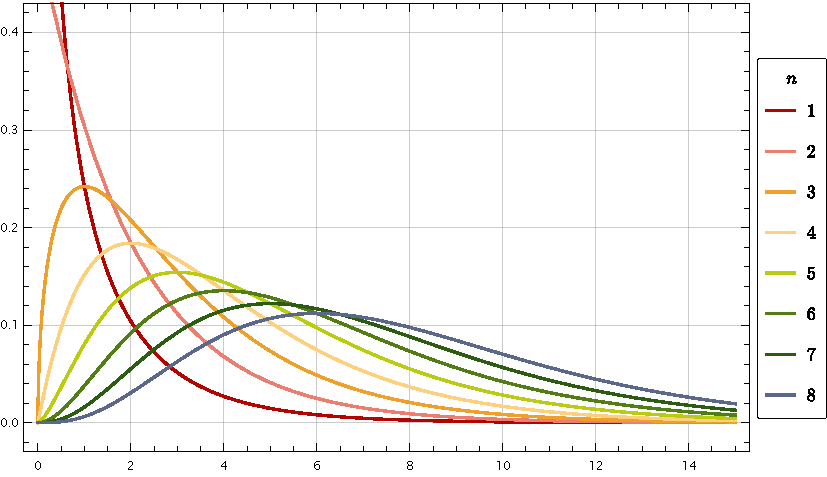
\includegraphics[scale=0.75]{Mathematica/output/Chi.pdf}
\end{Figure}

卡方分布有一些性质,我们罗列如下。
\begin{BoxProperty}[卡方分布的可加性]
    设$\chi_1^2\sim\chi^2(n_1), \chi_2^2\sim\chi^2(n_2)$,并且$\chi_1^2,\chi_2^2$相互独立,则有
    \begin{Equation}
        \chi_1^2+\chi_2^2\sim\chi^2(n_1+n_2)
    \end{Equation}
\end{BoxProperty}

\begin{BoxProperty}[卡方分布的期望和方差]
    设$\chi^2\sim\chi^2(n)$,则有
    \begin{Equation}
        E(\chi^2)=n\qquad
        D(\chi^2)=2n
    \end{Equation}
\end{BoxProperty}

\begin{BoxDefinition}[卡方分布的上分位数]
    对于给定的正数$\alpha$,$0<\alpha<1$,满足条件\footnote[2]{这里$\chi^2_{\alpha}(n)$就是一个带了些花里胡哨装饰的常数。}
    \begin{Equation}
        P\qty{\chi^2>\chi^2_{\alpha}(n)}=\Int[\chi_\alpha^2(n)][\infty]f(y)\dd{y}=\alpha
    \end{Equation}
    那么$\chi^2_{\alpha}(n)$就是$\chi^2(n)$分布的上$\alpha$分位数。
\end{BoxDefinition}

卡方分布的上$\alpha$分位数可以查表得到,当$n$充分大时,有以下近似公式
\begin{BoxFormula}[卡方分布的上分位数的近似]*
    卡方分布$\chi^2(n)$的上$\alpha$分位数$\chi_\alpha^2(n)$在$n$充分大时($n>40$),可以近似表示为
    \begin{Equation}
        \chi_\alpha^2(n)=\frac{1}{2}\qty(z_\alpha+\sqrt{2n-1})^2
    \end{Equation}
    其中$z_\alpha$是标准正态分布的上$\alpha$分位数。
\end{BoxFormula}

\subsubsection{学生氏分布}
\begin{BoxDefinition}[学生氏分布]*
    设$X\sim N(0,1)$,而$Y\sim\chi^2(n)$,且$X,Y$相互独立,则称随机变量$\chi^2$
    \begin{Equation}
        t=\frac{X}{\sqrt{Y/n}}
    \end{Equation}
    服从自由度为$n$的\uwave{学生氏分布}($t$分布),记为
    \begin{Equation}
        t\sim t(n)
    \end{Equation}
\end{BoxDefinition}

我们可能会很疑惑,为什么$t$分布被冠以“学生氏分布”这样一个奇怪的名字?$t$分布是由威廉·戈塞发现的,由于其发表相关论文时使用了“学生(Student)”的笔名,故得名如此。

\begin{Figure}[学生氏分布]
    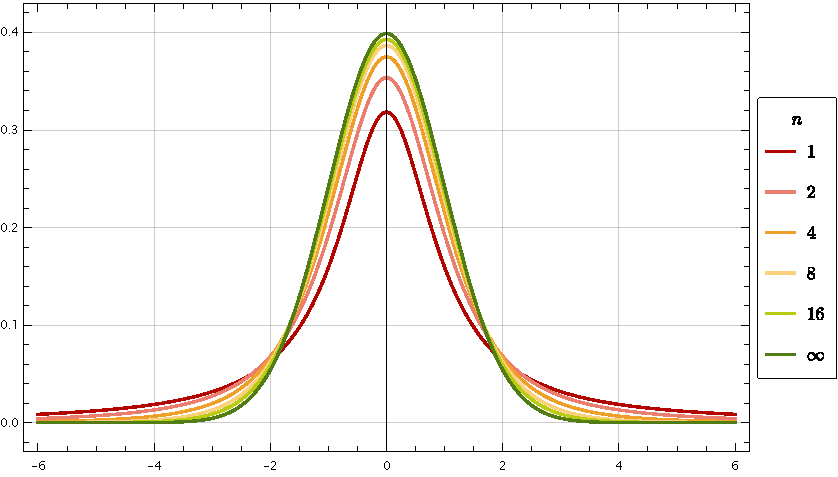
\includegraphics[scale=0.75]{Mathematica/output/Stu.pdf}
\end{Figure}

\begin{BoxFormula}[学生氏分布的概率密度]
    学生氏分布$t(n)$的概率密度为
    \begin{Equation}
        f(t)=\frac{\Gamma[(n+1)/2]}{\sqrt{n\pi}\Gamma(n/2)}\qty(1+\frac{t^2}{n})^{-(n+1)/2}\qquad -\infty<t<\infty
    \end{Equation}
\end{BoxFormula}

\begin{Proof}
    证明从略。
\end{Proof}

学生氏分布的概率密度函数如\xref{fig:学生氏分布}所示,可以证明,当$n$很大时$t(n)$会趋于$N(0,1)$

\begin{BoxDefinition}[学生氏分布的上分位数]
    对于给定的正数$\alpha$,$0<\alpha<1$,满足条件
    \begin{Equation}
        P\qty{t>t_{\alpha}(n)}=\Int[t_\alpha(n)][\infty]f(t)\dd{t}=\alpha
    \end{Equation}
    那么$t_{\alpha}(n)$就是$t(n)$分布的上$\alpha$分位数。
\end{BoxDefinition}

如\xref{fig:学生氏分布}所示,$t(n)$的概率密度函数$f(t)$是偶函数的,因此,如果上$\alpha$分位数取在正半轴的某个位置,那么上$1-\alpha$分位数就一定取在负半轴的相应位置,这就是说
\begin{BoxProperty}[学生氏分布的上分位数]
    学生氏分布的上分位数满足
    \begin{Equation}
        t_\alpha(n)=-t_{1-\alpha}(n)
    \end{Equation}
\end{BoxProperty}
学生氏分布的上$\alpha$分位数在$n$较大时,可以直接取用正态近似的结果。
\begin{BoxFormula}[学生氏分布的上分位数的近似]
    学生氏分布$t(n)$的上$\alpha$分位数$t_\alpha(n)$在$n$充分大时($n>45$),可以近似表示为
    \begin{Equation}
        t_\alpha(n)=z_\alpha
    \end{Equation}
    其中$z_\alpha$是标准正态分布的上$\alpha$分位数。
\end{BoxFormula}

\subsubsection{F分布}
\begin{BoxDefinition}[F分布]
    设$U\sim\chi^2(n_1)$,而$V\sim\chi^2(n_2)$,且$U,V$相互独立,则称随机变量
    \begin{Equation}
        F=\frac{U/n_1}{V/n_2}
    \end{Equation}
    服从自由度为$n$的\uwave{F分布},记为
    \begin{Equation}
        F\sim F(n_1,n_2)
    \end{Equation}
\end{BoxDefinition}

F分布描述的是两个服从卡方分布$\chi_1^2(n_1),\chi^2(n_2)$的随机变量除以其自由度$n_1,n_2$的比值。

F分布有一个显而易见的性质,即若$F\sim F(n_1,n_2)$,则
\begin{Equation}
    \frac{1}{F}\sim F(n_2,n_1)
\end{Equation}

\begin{BoxFormula}[F分布的概率密度]
    F分布$F(n_1,n_2)$的概率密度为(令$y=F$)
    \begin{Equation}
        f(y)=\frac{\Gamma[(n_1+n_2)/2](n_1/n_2)^{n_1/2}y^{(n_1/2)-1}}{\Gamma(n_1/2)\Gamma(n_2/2)[1+(n_1y/n_2)]^{(n_1+n_2)/2}}\qquad y>0
    \end{Equation}
\end{BoxFormula}

\begin{BoxDefinition}[F分布的上分位数]
    对于给定的正数$\alpha$,$0<\alpha<1$,满足条件
    \begin{Equation}
        P\qty{F>F_{\alpha}(n_1,n_2)}=\Int[F_\alpha(n_1,n_2)][\infty]f(y)\dd{y}=\alpha
    \end{Equation}
    那么$F_{\alpha}(n_1,n_2)$就是$F(n_1,n_2)$分布的上$\alpha$分位数。
\end{BoxDefinition}

\begin{BoxProperty}[F分布的上分位数]
    F分布的上分位数满足
    \begin{Equation}
        F_{\alpha}(n_1,n_2)=\frac{1}{F_{1-\alpha}(n_1,n_2)}
    \end{Equation}
\end{BoxProperty}
